% Main file for Overleaf. Compile with pdfLaTeX; references use BibTeX.
% All manuscript text is here; figures/ contains only the vector PDFs used below.
% The local conference, bibliography, and dependency files preserve the submission style.
\documentclass{article}
\usepackage{iclr2027_conference,times}
% Use default hyperlink borders; do not add bold citation formatting.
\usepackage{hyperref}
\usepackage{url}
\usepackage{booktabs}
\usepackage{amsmath,amssymb}
\usepackage{graphicx}
\usepackage{xcolor}
\usepackage{microtype}

% Manuscript metadata.
\title{One Set of Weights, Many Algorithms:\\How Looped Transformers Route Computation\\Across Loops}
\author{Anonymous authors}

% Subfigure labels are maintained in LaTeX, including panels with no printed caption.
\usepackage{subcaption}
\begin{document}
\maketitle

\begin{abstract}
Looped Transformers provide a recurrent architecture for latent reasoning by repeatedly using the same set of Transformer layers.
As the hidden state evolves from one loop to the next, the same weights operate on different states, so parameter sharing alone does not determine the task-level computation performed at each loop.
This leaves open how the shared layers are reused across loops and what determines the computation they perform at each loop.

We first show that repeated use of the same layers need not imply fixed task progress.
We then demonstrate that affine steering of the entering hidden state can redirect the next frozen loop toward different targets.
We further trace this control to attention routing: patching steered attention patterns into an unsteered run recovers much of the steering effect.
Finally, we characterize how steering depends on execution depth, backbone supervision, and controller capacity.
\end{abstract}

% --- Introduction ---
\section{Introduction}
\label{sec:intro}

Latent reasoning studies how models can perform multi-step computation in their hidden states without generating every intermediate step as text \citep{saunshi2025looped,geiping2025scaling}. Recurrent architectures provide a natural way to perform this computation. They repeatedly apply the same transformation to an evolving hidden state, rather than adding a new set of layers for each step \citep{dehghani2019universal}. When the shared transformation consists of Transformer layers, the architecture is called a Looped Transformer \citep{yang2024learning,fan2025looped}. Running more loops increases computation without increasing the number of parameters. Research on these models shows why this extra computation can be useful. Looped Transformers can learn iterative learning algorithms efficiently \citep{yang2024learning}, and recurrent depth can increase their capacity for reasoning \citep{saunshi2025looped}. Adaptive looping also improves length generalization on tasks with iterative solutions \citep{fan2025looped}. At language-model scale, Huginn and Ouro use recurrent depth to support latent computation and adjust the amount of test-time compute \citep{geiping2025scaling,zhu2025ouro}. These results make repeated use of shared layers a practical approach to extending computation within hidden states.

Weight sharing creates the intuition that each loop makes the same amount of progress on the task. In graph traversal, for example, each loop would move one step along the graph. Indeed, looped Transformers can be programmed to execute iterative algorithms with fixed weights \citep{giannou2023loops}. But the existence of such a construction does not mean that end-to-end training will learn the same algorithm. Shared weights fix the network transformation, but the hidden state entering it changes across loops. The task-level operation may depend on that state. For example, the same block could advance along a path in one state and preserve an answer in another. Training on final answers does not require the model to follow a prescribed sequence of intermediate steps. In trained looped models, individual layers can approach distinct fixed points while the shared block follows a cyclic hidden-state trajectory \citep{blayney2026mechanistic}. Probing studies also find limited evidence of directly readable intermediate reasoning steps \citep{lu2025probing}. These findings leave unclear how repeated use of the same layers translates into progress on a task. Shared weights alone do not tell us whether each loop advances by the same amount.

We begin with readouts at intermediate loops to examine how shared layers advance a task. We then move from observing this progress to controlling the next target and identifying the mechanism that carries the change. Figure~\ref{fig:mechanism} summarizes these three findings.

\textbf{Phenomenon: shared weights do not imply fixed task progress.} Intermediate readouts can advance at different rates or remain at an already reached target, as illustrated at the top of Figure~\ref{fig:mechanism}. A learned loop therefore need not correspond to one task step (Section~\ref{sec:underdetermined}).

\textbf{Control: the entering state can redirect the next target of a frozen loop.} As illustrated at the bottom left of Figure~\ref{fig:mechanism}, different affine maps steer the same state toward different next targets without changing the network weights or loop budget (Section~\ref{sec:target}).

\textbf{Mechanism: attention routing carries much of this target redirection.} The bottom right of Figure~\ref{fig:mechanism} shows that steering changes where attention reads, and patching these attention patterns recovers much of the steering effect (Section~\ref{sec:hypothesis}).

Further, we study the generalization and limits of state steering across backbone supervision strategies and steering-map capacities (Section~\ref{sec:generalization}).

% Figure 1: supplied overview; respect its PDF crop box.
\begin{figure}[!htbp]
  \centering
  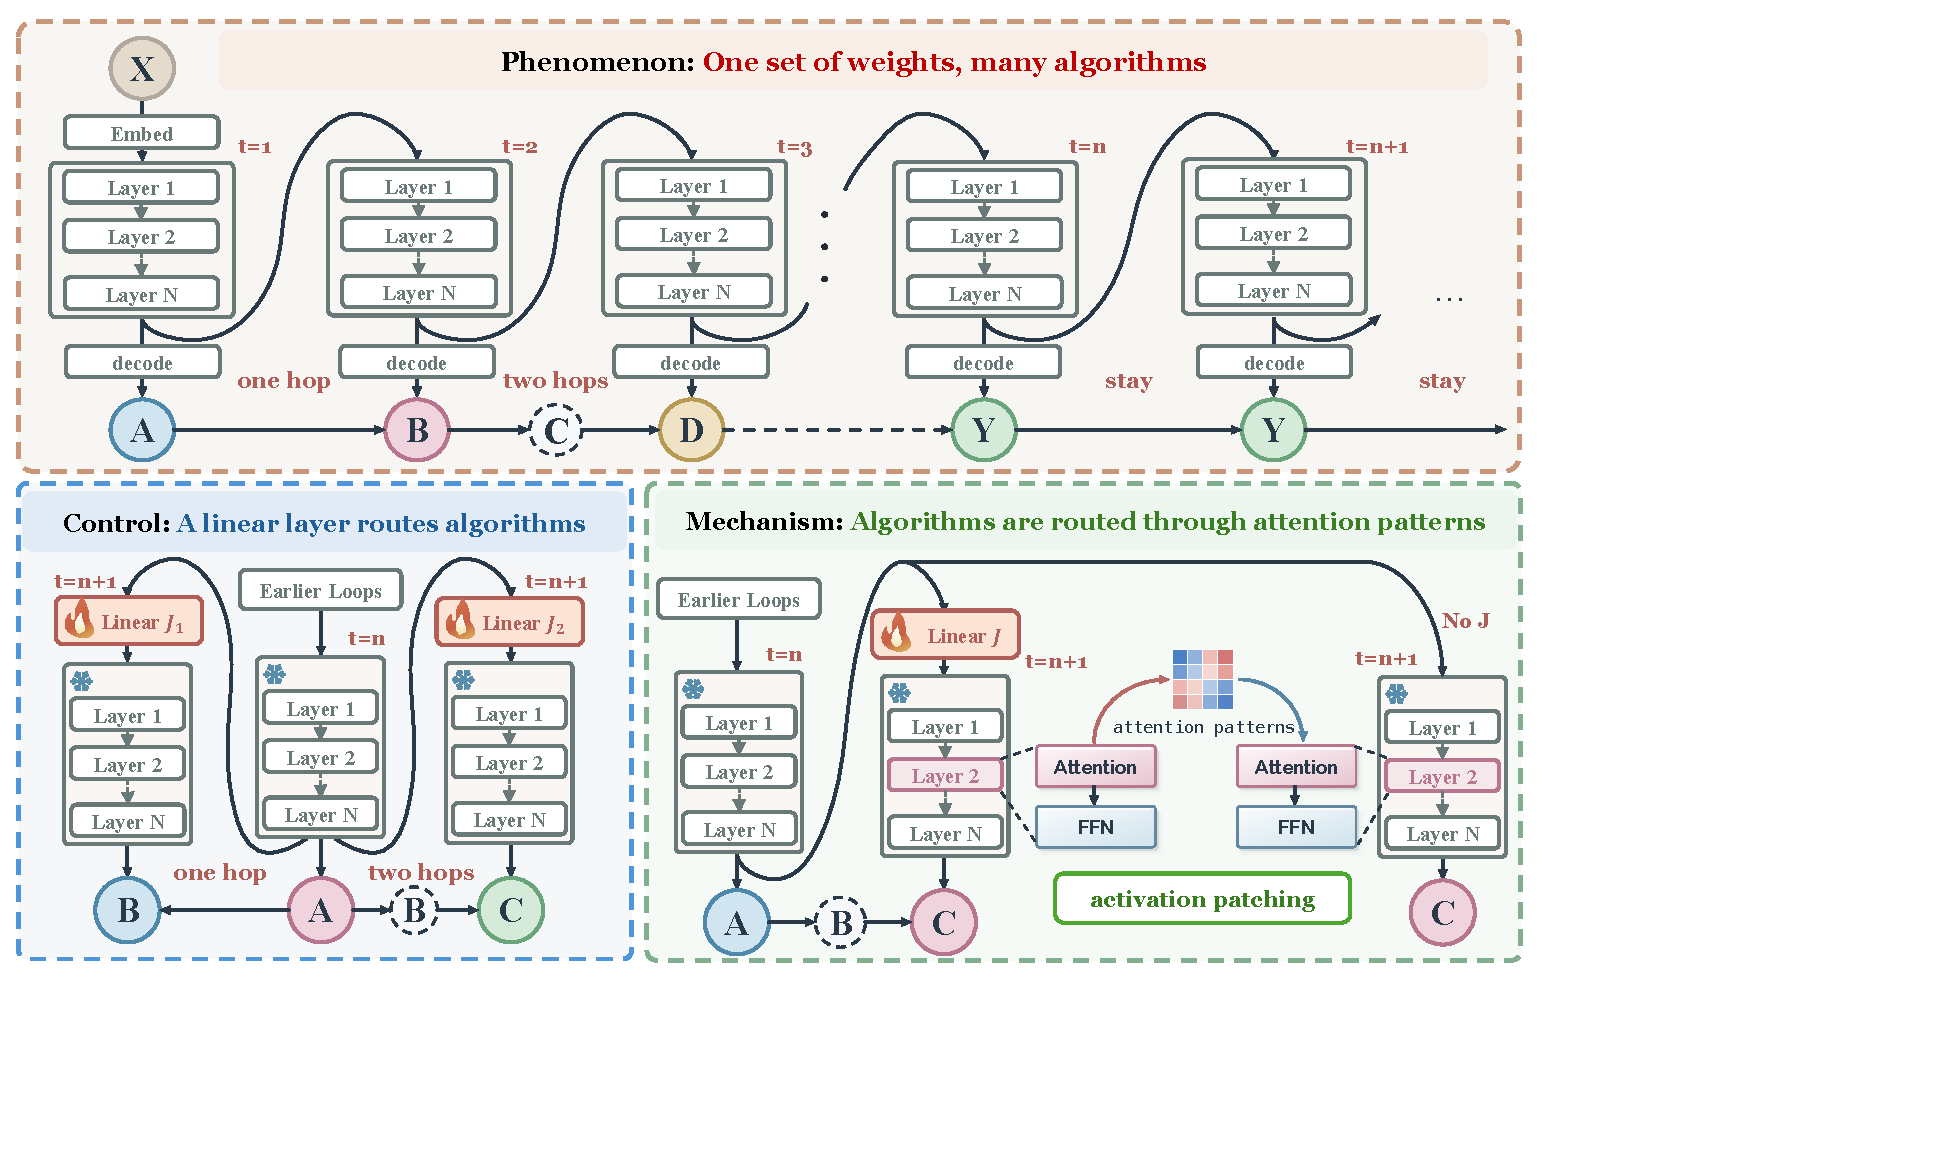
\includegraphics[pagebox=cropbox,width=\linewidth]{figures/fig01_overview.pdf}
  \caption{
\textbf{One set of weights, different targets of computation.}
Top: repeating the same shared block does not enforce a fixed relation between loop number and task progress; intermediate readouts can advance at different rates or remain at an already reached target.
Bottom left: learned affine maps $J_1$ and $J_2$ redirect the same entering state toward different next targets while the recurrent backbone remains frozen.
Bottom right: patching attention patterns from a steered run into an unsteered run tests whether attention routing carries this target redirection.
Flames denote trainable steering maps; snowflakes denote frozen network blocks.
}
\label{fig:mechanism}
\end{figure}

% --- Related Work ---
\section{Related Work}
\label{sec:related}

\paragraph{Looped Transformers.}
Looped Transformers are one approach to reasoning within hidden states \citep{zhu2025survey,li2025implicit}. Research on these models addresses three broad questions. The first is what shared layers can compute and learn. These studies examine which computations recurrent architectures can express and which algorithms fixed-weight looped Transformers can execute \citep{dehghani2019universal,giannou2023loops}. Learning studies examine whether training can recover iterative algorithms, including multi-step optimization \citep{yang2024learning,gatmiry2024gradient}. The second is whether additional loops improve reasoning and generalization beyond training \citep{saunshi2025looped,fan2025looped,soulos2024recurrent}. The third is how to use recurrent depth at scale. Large recurrent language models use loops for additional test-time computation \citep{geiping2025scaling,zhu2025ouro}. Related methods learn when to stop, allocate depth adaptively, or stabilize computation over longer runs \citep{yang2026stabilizing,movahedi2026fixed,popescu2026adaptive}.

\paragraph{Mechanistic studies of looped computation.}
Mechanistic work studies how trained models use their loops. One direction examines what can be read from intermediate states and what supervision leaves unconstrained \citep{lu2025probing,fan2026lotus,sharma2026readout}. Another studies how hidden states evolve across depth, identifying fixed points, cyclic trajectories, repeated inference stages, and distinct dynamical phases \citep{blayney2026mechanistic,kapl2026growing,kim2026phase}. This work also includes causal interventions. \citet{zhang2026recurrence} relate training budgets to per-loop progress and test that progress through activation patching. \citet{popescu2026adaptive} fit exit gates to frozen trajectories, separating the computation that produces a trajectory from the decision to stop. Other work studies key and value representations and finds low-rank structure in their changes across loops \citep{oneill2026looped}. These studies examine both the organization of recurrent computation and ways to control its execution.

\paragraph{State steering and attention intervention.}
Activation steering changes model behavior by modifying hidden activations \citep{turner2023activation}. Affine steering provides a learned linear transformation with a bias for this purpose \citep{singh2024surgery}. Activation patching tests the role of internal components by replacing their activations with those from another run \citep{wang2023ioi}. We use these tools to study target selection within a trained, frozen loop. Different state interventions select different next targets, and attention patches test how the change is carried through the network. Reusing the learned map across loops then lets us examine how long this control lasts.

% --- Phenomenon: Task Progress Varies across Loops ---
\section{Phenomenon: Task Progress Varies across Loops}
\label{sec:underdetermined}
A natural view of a looped Transformer is that each loop repeats the same task-level step. Weight sharing alone, however, does not specify how far each loop advances toward the answer. We examine this relation between loop number and task progress using graph traversal. Each input specifies a directed graph $G$ in which every node has exactly one successor, a starting node $s$, and a path length $k$. Let $f_G(v)$ denote the successor of node $v$. The model must predict $f_G^k(s)$, the node reached after $k$ graph edges. Reading out a predicted node after each loop lets us track progress along the graph. Appendix~\ref{app:graph-task} gives the input-token format, supervision, and examples.

The models reuse a two-layer Transformer block. We denote each configuration by $D_mL_n$, where $m$ is the maximum graph-traversal depth used in training and $n$ is the number of training loops. Both D8L8 and D8L6 are trained on path lengths 1--8, using eight and six loops, respectively. Only the answer at the final loop is supervised. Intermediate readouts are not supervised, so training does not specify which node the model should predict at each earlier loop.

At evaluation time, we keep the trained parameters fixed and repeatedly apply the same shared block for 16 loops, beyond the eight or six loops used in training. This lets us observe whether the model keeps predicting the target or moves past it after the final supervised loop. We request the eight-hop target and read out predictions at loops 0--16. Loop 0 denotes the state before the first application of the shared block. Each model is evaluated on 512 held-out ten-node cycles with all ten starting nodes, giving 5,120 examples. Figure~\ref{fig:trajectory} shows four examples from twelve D8L8 and five D8L6 runs. Rows correspond to loops, and columns correspond to nodes along the path. Each row shows how often the model predicts each node.

% Figure 2: four vector panels. Unequal widths compensate for different axis margins; keep labels below panels.
\begin{figure}[!htbp]
\centering
\captionsetup[subfigure]{hypcap=true,labelformat=parens,justification=centering}
\setcounter{subfigure}{0}%
\begin{subfigure}[t]{0.27625\linewidth}
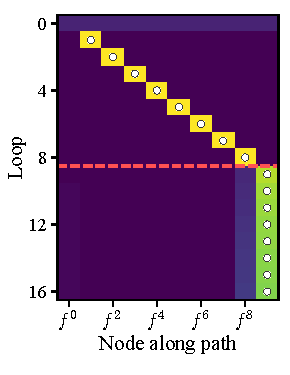
\includegraphics[width=\linewidth]{figures/fig02a_readout.pdf}
\caption{D8L8}\label{fig:trajectory-a}
\end{subfigure}%
\begin{subfigure}[t]{0.23250\linewidth}
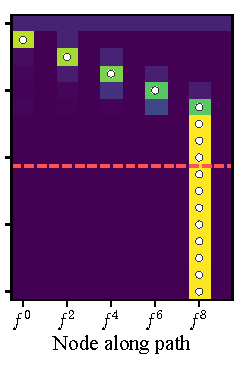
\includegraphics[width=\linewidth]{figures/fig02b_readout.pdf}
\caption{D8L8}\label{fig:trajectory-b}
\end{subfigure}%
\begin{subfigure}[t]{0.23250\linewidth}
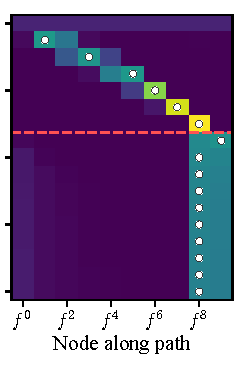
\includegraphics[width=\linewidth]{figures/fig02c_readout.pdf}
\caption{D8L6}\label{fig:trajectory-c}
\end{subfigure}%
\begin{subfigure}[t]{0.25875\linewidth}
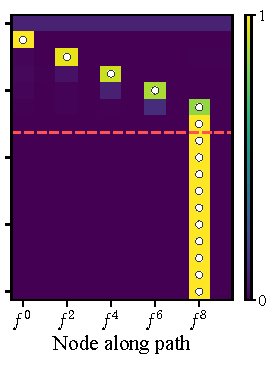
\includegraphics[width=\linewidth]{figures/fig02d_readout.pdf}
\caption{D8L6}\label{fig:trajectory-d}
\end{subfigure}%
\caption{Intermediate readouts; color shows prediction frequency. Red dashed lines mark the last supervised loop; white dots mark the unique most frequent prediction.}
\label{fig:trajectory}
\end{figure}

Before reaching the target, the readouts advance at different rates. In Figure~\ref{fig:trajectory-a}, the most frequent prediction advances one node per loop. In Figure~\ref{fig:trajectory-b}, it first stays at the starting node and then advances mainly two nodes at a time. The two D8L6 models both reach the target in six loops, but follow different intermediate readout trajectories (Figures~\ref{fig:trajectory-c} and~\ref{fig:trajectory-d}). Thus, even models trained with the same loop budget need not predict the same intermediate nodes.

After the final supervised loop, the readouts also differ. Some models continue to predict the target, while others predict nodes beyond it. Repeating the shared block therefore does not necessarily advance the decoded answer: it can also preserve an answer already reached.

These results show that shared weights and final-answer supervision do not impose a fixed relation between loop number and graph hops. The readouts identify the predicted node at each loop, rather than the hidden operations that produce it. We next test whether the entering hidden state can control the next target of a frozen loop. The target-selection and main graph mechanism experiments use the same D8L6 backbone.

% --- Control: State Steering Redirects the Next Target of a Frozen Loop ---
\section{Control: State Steering Redirects the Next Target of a Frozen Loop}
\label{sec:target}
Section~\ref{sec:underdetermined} shows that shared weights can produce different readout trajectories. We now test whether changing the entering hidden state can control the next target of a trained loop. We learn affine maps $J$ for different targets and apply them to the same starting state. The network weights and loop budget remain fixed.

\subsection{State Steering with a Frozen Backbone}
A loop applies a shared block of Transformer layers to the current hidden states. Each layer has its own attention and feed-forward parameters; some architectures use a mixture-of-experts module in place of the feed-forward network. The entire block is reused across loops. Let $F$ denote this block and $h_t$ the sequence of token hidden states after loop $t$. The recurrence is
\begin{equation}
 h_{t+1}=F(h_t), \qquad t=1,2,\ldots.
\end{equation}

For affine steering, we apply the same learned affine map $J$ independently to each token's hidden state before the next shared block. It changes the entering states without mixing information across tokens. We call the frozen network the backbone. During steering training, we update only $J$. The backbone then processes the transformed states to produce the next output.

\subsection{Selecting One-Hop and Two-Hop Targets}
Figures~\ref{fig:trajectory-c} and~\ref{fig:trajectory-d} show that D8L6 readouts can advance by one or two graph hops in a single loop. This suggests that the shared block has learned computation that can advance multiple steps along the graph. We now test whether $J$ can control this computation so that the next frozen loop advances by one or two hops as requested.

We freeze the D8L6 backbone and train two affine maps. Each map uses a diagonal term plus a rank-48 low-rank term. Both maps act on the same hidden state. We use $u=f_G^8(s)$ as the start node for continuation. We train $J_{\mathrm{one}}$ so that the next frozen loop predicts $f_G(u)$, one hop beyond $u$. We train $J_{\mathrm{two}}$ so that it predicts $f_G^2(u)$, two hops beyond $u$. Appendix~\ref{app:target-setup} gives the detailed configuration.

% Figure 3: accuracy and PCA panels; empty captions print only the (a)/(b) labels.
\begin{figure}[!htbp]
\centering
\captionsetup[subfigure]{hypcap=true,labelformat=parens,labelsep=none,justification=centering}
\setcounter{subfigure}{0}%
\begin{subfigure}[t]{.60\linewidth}
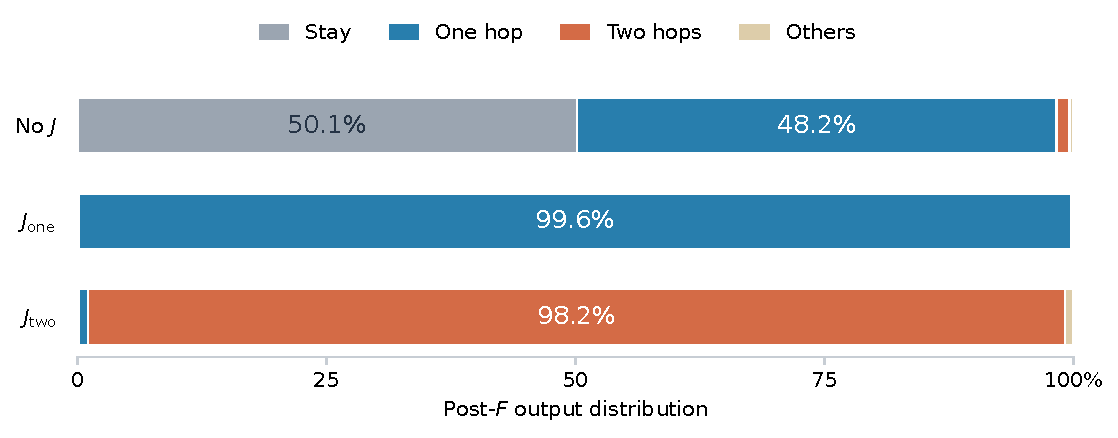
\includegraphics[width=\linewidth]{figures/fig03a_target_accuracy.pdf}
\caption{}\label{fig:target-behavior}
\end{subfigure}\hfill
\begin{subfigure}[t]{.38\linewidth}
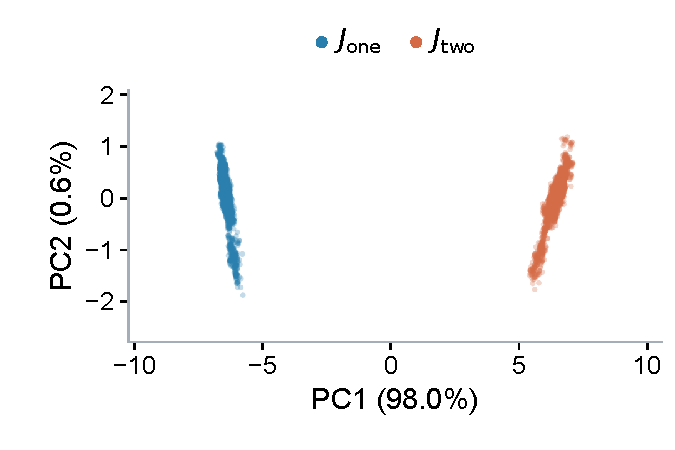
\includegraphics[width=\linewidth]{figures/fig03b_pca.pdf}
\caption{}\label{fig:target-pca}
\end{subfigure}

\caption{(a) Output-node matching accuracy after $F$. (b) PCA of token-averaged hidden states before $F$, after the one-hop and two-hop maps.}
\label{fig:target}
\end{figure}

Figure~\ref{fig:target-behavior} shows that the two maps direct the next frozen loop toward their respective targets. The maps change the predicted continuation while leaving the input graph and its successor relation unchanged. This control generalizes to graphs excluded from map training, so it does not depend on memorizing the training graphs.

The two maps produce visibly separated groups of entering states in the shared PCA projection (Figure~\ref{fig:target-pca}). Appendix~\ref{app:target-pca} gives the projection method.

Table~\ref{tab:steering-scope} summarizes our further tests of state steering. Each experiment keeps the backbone fixed and trains only the controller.

\begin{table}[!htbp]
\centering
\caption{Further experiments on state control.}
\label{tab:steering-scope}
\footnotesize
\setlength{\tabcolsep}{3pt}
\renewcommand{\arraystretch}{1.05}
\begin{tabular*}{\linewidth}{@{\extracolsep{\fill}}lll@{}}
\toprule
Task & Form of $J$ & Focus \\
\midrule
Ouro letter-walk & Dense affine & Routing mediation of steering (\S\ref{sec:hypothesis}) \\
Parity & Diagonal + low-rank ($r=48$) & Readout timing at longer lengths (\S\ref{sec:depth-boundary}) \\
Graph continuation & Diagonal + low-rank ($r=48$) & Control beyond the fitted loops (\S\ref{sec:depth-boundary}) \\
Ouro cancellation & Residual affine ($r=128$) & Effect of backbone supervision (\S\ref{sec:supervision-boundary}) \\
KG composition & Low-rank affine, dense affine, MLP, attention & Capacity for longer compositions (\S\ref{sec:complexity-boundary}) \\
\bottomrule
\end{tabular*}
\end{table}

These experiments examine state control across graph, language, and parity tasks. We first study how attention routing carries this control in graph traversal and Ouro letter-walk. We then examine its limits across the remaining tasks.

% --- Mechanism: Attention Routing Carries the Steering Effect ---
\section{Mechanism: Attention Routing Carries the Steering Effect}
\label{sec:hypothesis}\label{sec:large}
Section~\ref{sec:target} shows that we can control the next target of a frozen loop. We now study the mechanism behind this control. In graph traversal and Ouro letter-walk, attention routing carries much of the effect by changing where the network reads.

For graph traversal, we reuse the frozen D8L6 backbone and one-hop maps from Section~\ref{sec:target}. We also test Ouro-2.6B on \emph{letter-walk}. Each input lists who passes a letter to whom and names the person who starts with it. At each step, the current holder passes the letter to the next person specified in the input. For example, if Alice passes to Bob and Bob passes to Carol, a letter starting with Alice reaches Carol after two steps. The model is asked who has the letter after a given number of steps and outputs that person's name. Appendix~\ref{app:parallel} gives prompt examples, tokenization, and supervision details.

We first fine-tune Ouro on questions that require following the letter for 1--4 steps. We use four loops and supervise only the answer at loop 4. We then freeze the backbone and train a dense affine $J$ on questions that require 1--8 steps, again supervising the answer at loop 4. Unlike the graph controller's low-rank parameterization, this map uses an unrestricted weight matrix and a bias. The same $J$ acts independently on every token before loops 2--4. The model therefore learns to follow the letter for more steps while the backbone and four-loop budget stay fixed. Training configurations are given in Appendices~\ref{app:target-setup} and~\ref{app:ouro-config}; head selection and evaluation protocols are given in Appendices~\ref{app:n10-mechanism} and~\ref{app:ouro-evaluation}.

% Figure 4: one composite vector PDF contains the attention schematic and three result panels.
\begin{figure}[!t]
\centering
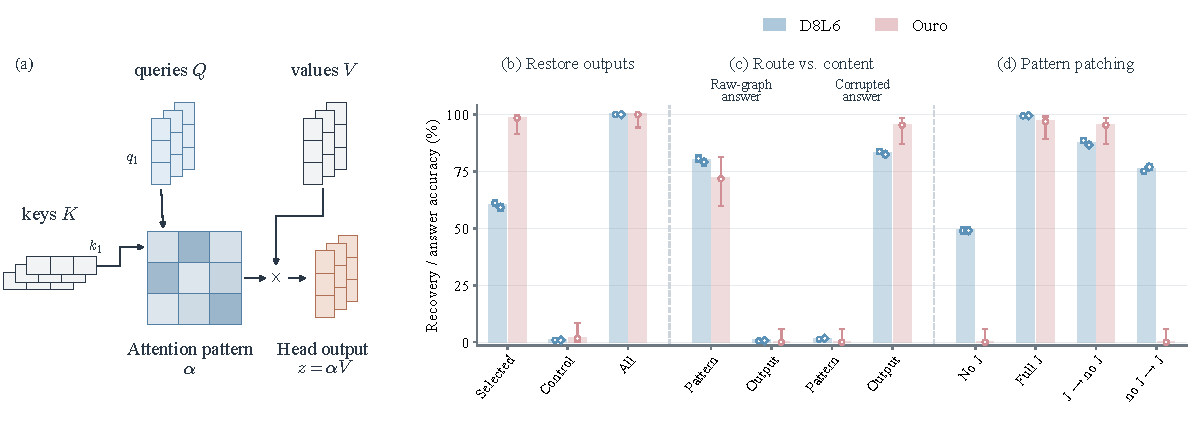
\includegraphics[width=\linewidth]{figures/fig04_attention_mechanism.pdf}
\caption{(a) Attention schematic. (b--d) Attention-intervention results in D8L6 and Ouro.}
\label{fig:parallel-mechanism}\label{fig:causal}\label{fig:restore}\label{fig:routing-swap}
\end{figure}

\subsection{Restoring Head Outputs Recovers Answers}
\label{sec:restore}
We first test whether selected attention heads supply information that the model uses to answer. Each head assigns attention weights to token positions and combines the value vectors at those positions into a head output (Figure~\ref{fig:parallel-mechanism}a). We disrupt this computation, then test whether restoring the selected head outputs restores the answer.

We run the same graph with two different starting nodes. The original run provides the clean answer and head outputs. The alternative run provides replacement queries. We insert these queries into the original run while keeping its keys and values unchanged. This changes where attention reads without replacing the input's value vectors. We then replace the selected heads' disrupted outputs with their clean outputs and let the model continue. For an intervened head, let $Q_{\mathrm{alt}}$ denote the replacement queries and $d_k$ the query/key dimension:
\begin{equation}
 z_{\mathrm{broken}}
 =\operatorname{softmax}\!\left(\frac{Q_{\mathrm{alt}}K_{\mathrm{clean}}^\top}{\sqrt{d_k}}\right)V_{\mathrm{clean}},
 \qquad
 z_{\mathrm{restored}}\leftarrow z_{\mathrm{clean}},
\end{equation}
Here softmax is taken over the visible key positions. If the selected outputs carry information needed for the answer, restoring them should repair the error caused by query replacement. We compare this repair with restoring a control set of heads. Recovery is measured only on examples that were answered correctly before query replacement and incorrectly afterward.

Figure~\ref{fig:parallel-mechanism}b shows that restoring the selected outputs repairs answers in both models. In D8L6, it repairs 60.1\% of disrupted answers, compared with 0.9\% for the control. In Ouro, it repairs 62 of 63 answers, while the matched control repairs one. Restoring all affected outputs recovers every disrupted answer in both models. The selected head outputs therefore supply information that the later computation uses to produce the answer.

\subsection{Pattern and Output Patches Select Different Answers}
\label{sec:causal}
Restoring head outputs shows that attention supplies useful information, but does not separate where the head reads from what it retrieves. We separate these effects by comparing two patches. A pattern patch copies attention weights while retaining the receiving run's value vectors. An output patch copies the source head's weighted combination of values instead.

We construct two inputs with aligned token positions but different graphs and starting nodes. One run supplies the patch; the other receives it. Consider a position that contains node D in the source input but node C in the receiving input. If the source pattern directs attention to this position, copying that pattern should favor C, because the receiving values still encode the receiving graph. Copying the source head output should instead favor D. We choose examples in which C, D, and the original receiving answer are all distinct. This makes the two predicted effects distinguishable from each other and from leaving the answer unchanged. Ouro uses the same construction with letter-walk descriptions.

Let $\alpha$ denote the attention pattern, $V$ the value vectors, and $z=\alpha V$ the head output. We apply the two patches separately:
\begin{equation}
 z_{\mathrm{pattern\ patch}}=\alpha_{\mathrm{source}}V_{\mathrm{receiver}},
 \qquad
 z_{\mathrm{output\ patch}}=z_{\mathrm{source}}.
\end{equation}
In both cases, the receiving run continues from the patched activation. The difference is whether it receives the source's attention weights or the source's retrieved output.

Figure~\ref{fig:parallel-mechanism}c shows the predicted separation. Pattern patches favor the answer obtained by reading the receiving graph at the source-selected positions: C in the example above. They produce this answer in 79.8\% of D8L6 cases and 71.9\% of Ouro cases. Output patches instead favor the source answer, D, in 83.2\% and 95.3\% of cases, respectively. Thus, changing where a head reads can redirect the answer without copying the source head's retrieved content.

\subsection{Attention Patterns Carry the Steering Effect}
\label{sec:routing}\label{sec:qkv}
The previous experiment shows that attention patterns can redirect an answer. We now test whether changes in these patterns carry the effect of $J$. Unlike the previous experiment, the two runs receive exactly the same input. One uses $J$ and the other does not.

We copy attention patterns from the steered run into selected heads of the unsteered run. The unsteered run keeps its own value vectors and continues without applying $J$. If routing carries the steering effect, this patch should move its accuracy toward that of the steered run. We also test the reverse direction: copying unsteered patterns into the steered run should reduce its accuracy. Writing $J$ and $0$ for the steered and unsteered runs, respectively, the patched outputs are
\begin{equation}
 z_{J\rightarrow 0}=\alpha_J V_0,
 \qquad
 z_{0\rightarrow J}=\alpha_0 V_J.
\end{equation}
The arrow indicates which run supplies the pattern and which receives it. In each direction, only the pattern is copied; the receiving run retains its own values and steering schedule.

Both effects appear in Figure~\ref{fig:parallel-mechanism}d. In D8L6, copying steered patterns raises unsteered accuracy from 49.0\% to 87.6\%, compared with 99.4\% under full steering. This recovers 76.5\% of the steering gain, averaged across the two map fits. Copying unsteered patterns in the reverse direction reduces steered accuracy to 76.0\%. In Ouro, steered patterns raise unsteered accuracy from 0/64 to 61/64, close to 62/64 with full steering. The reverse patch reduces accuracy to 0/64. Attention patterns therefore carry a substantial part of the controller's effect: copying them recovers much of the gain without applying $J$ in the receiving run.

Together, these interventions show that attention routing carries much of the steering effect in graph traversal and Ouro letter-walk. Additional results are reported in Appendices~\ref{app:graph-results} and~\ref{app:ouro-results}.

% --- Generalization and Limits of State Steering ---
\section{Generalization and Limits of State Steering}
\label{sec:generalization}
The effect of steering depends on the task, training method, and model configuration. We explore further uses of $J$ across different tasks and settings, focusing on depth generalization, backbone supervision, and steering-map capacity. These experiments show how steering can be extended and where it remains limited.

\subsection{Depth Generalization across Tasks}
\label{sec:depth-boundary}\label{sec:parity}
We first compare graph traversal with parity. Given a binary sequence of length $n$, the parity task asks whether the number of ones is even or odd: $y=(\sum_{i=1}^{n}x_i)\bmod 2$. Following the setup of \citet{fan2025looped}, we read the answer after $t=n$ loops. We train the backbone on lengths 1--20, then freeze it and train a shared affine $J$ on lengths 20--40. Appendix~\ref{app:parity} gives the input-token format, supervision, examples, and detailed configuration.

The two tasks show different behavior beyond the range used to train $J$ (Figure~\ref{fig:boundary}). In the displayed parity run, steering maintains high accuracy at lengths approaching 200, although the backbone was trained only through length 20 and $J$ through length 40. In graph traversal, we train $J$ to maintain one-hop progress through loop 16. Accuracy drops substantially before loop 20, even though $J$ remains active. This decline occurs across twelve D8L8 backbones, separate from the D8L6 models used in the mechanism experiments. Appendix~\ref{sec:boundary} gives their configuration and per-seed results. Thus, the same strategy of reusing a learned map supports much longer execution in parity than in this graph task.

% Figure 5: two panels share the legend PDF below them. Phantom captions preserve panel references.
\begin{figure}[!htbp]
\centering
\setcounter{subfigure}{0}%
\begin{subfigure}[t]{.495\linewidth}
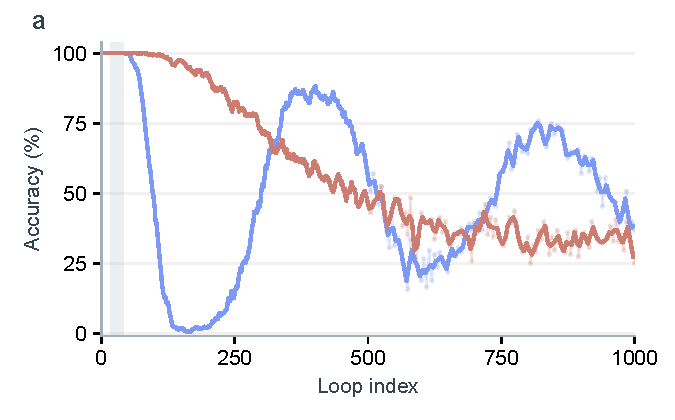
\includegraphics[width=\linewidth]{figures/fig05a_parity.pdf}
\phantomcaption\label{fig:v64-parity}
\end{subfigure}\hfill
\begin{subfigure}[t]{.495\linewidth}
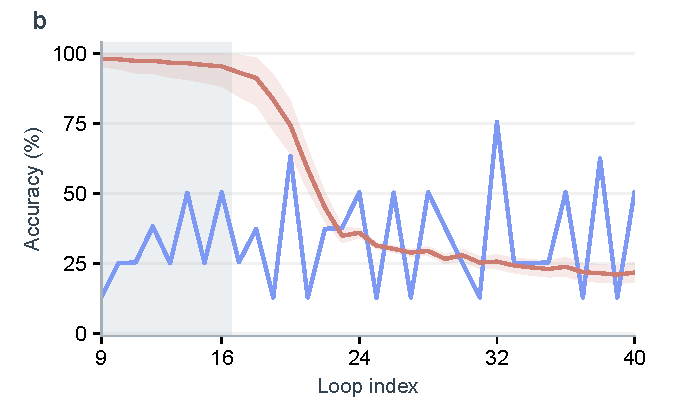
\includegraphics[width=\linewidth]{figures/fig05b_graph.pdf}
\phantomcaption\label{fig:v64-graph}
\end{subfigure}
\par\nointerlineskip

\includegraphics[width=\linewidth]{figures/fig05_legend.pdf}

\caption{Accuracy with and without steering on (a) parity and (b) graph continuation. Blue denotes no $J$; red denotes steering with $J$.}
\label{fig:boundary}
\end{figure}

To understand the parity result, we examine when the model produces the correct answer. Training ties input length $n$ to readout loop $t=n$. Accurate readouts should therefore follow a line with slope one in the length--loop plot. In the unsteered model, this slope is slightly different. The gap between the accurate readout and the requested loop grows with input length. This suggests a simple role for $J$: correcting readout timing so that accurate answers remain aligned with $t=n$.

Figures~\ref{fig:parity}a,b show this correction for seed 2. Near length 60, the unsteered accuracy band lies roughly half a loop before the requested schedule. With $J$, it stays closer to the diagonal. The best nearby integer-loop readout changes from $t=n-1$ to $t=n$.

% Figure 6: parity readout-timing composite.
\begin{figure}[!htbp]
\centering
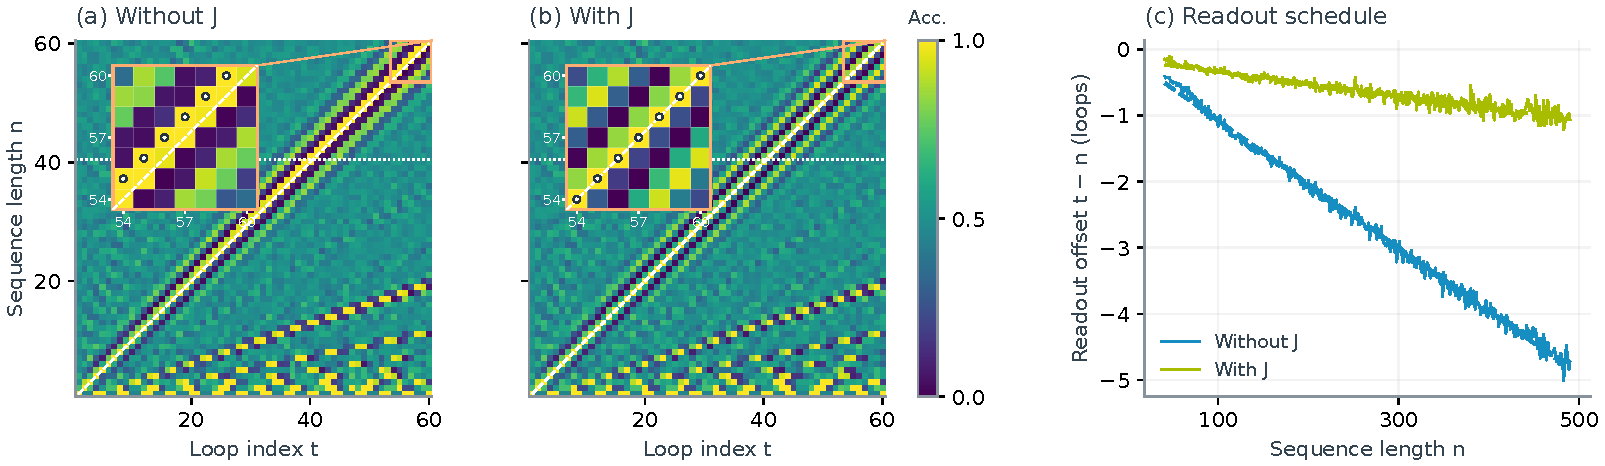
\includegraphics[width=\linewidth]{figures/fig06_parity_timing.pdf}
\caption{Parity readout timing for seed 2. (a,b) Accuracy across input length $n$ and loop $t$, without and with $J$; insets enlarge lengths 54--60. The diagonal marks $t=n$, and dots mark the best nearby integer loop. (c) Continuous readout offset $t-n$ and fitted trends across lengths 41--490.}
\label{fig:parity}\label{fig:parity-phase}
\end{figure}

We quantify this gap as $\Delta(n)=t_{\mathrm{read}}(n)-n$, where $t_{\mathrm{read}}$ estimates the position of the recurring accuracy band (Figure~\ref{fig:parity}c). The fitted slope of $t_{\mathrm{read}}(n)$ against $n$ increases from 0.9904 without $J$ to 0.9982 with $J$. Accordingly, the magnitude of the timing drift falls from 0.96 to 0.18 loops per 100 input tokens. This supports the timing explanation: training $J$ on lengths 20--40 reduces an error that would otherwise accumulate at longer lengths. Appendix~\ref{app:parity-evaluation} describes the estimator, and Appendix~\ref{app:parity-results} reports results for the other backbones.

\subsection{Steering under Different Backbone Supervision}
\label{sec:supervision-boundary}
We next test how backbone training affects the computation that steering can control. We use Ouro antonym cancellation. The input is a word sequence, and each task step deletes the leftmost adjacent antonym pair. The remaining words are joined without changing their order, which can create a new adjacent antonym pair. The model must name the pair removed at the requested step. Appendix~\ref{app:supervision} gives the text-input format, supervision, examples, and evaluation settings.

Our earlier experiments suggest that $J$ changes how the frozen loop uses its learned computation. Under this interpretation, steering should depend on what the backbone has learned. In particular, a state change should enable faster progress only if the backbone can perform the required computation. We test this prediction by comparing two supervision strategies.

Both backbones run for four loops. Stepwise supervision trains loop $t$ to report the pair removed at step $t$, for $t=1,\ldots,4$. Final-only supervision asks for a deletion step from 1--4 and trains the model to report that pair at loop 4. It does not supervise the earlier readouts. We first examine how these two strategies affect readouts before adding $J$.

% Figure 7: one composite PDF for supervision and controller comparisons.
\begin{figure}[!htbp]
\centering
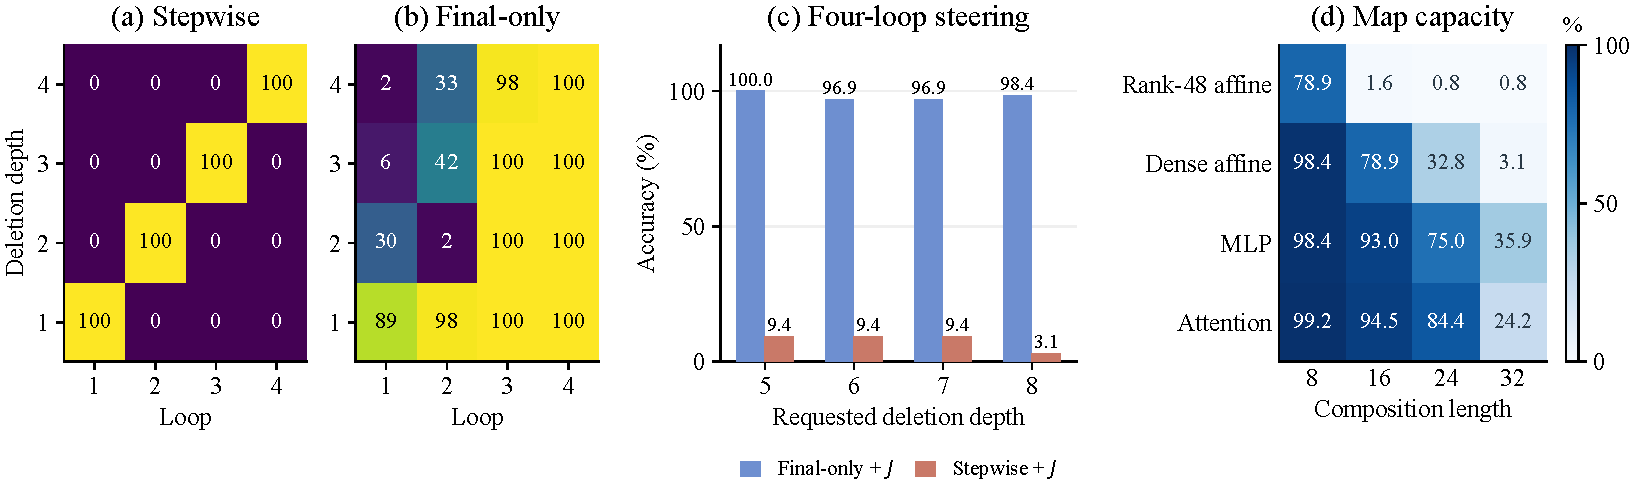
\includegraphics[width=\linewidth]{figures/fig07_supervision_capacity.pdf}
\caption{(a,b) Native Ouro readout accuracy under stepwise and final-only supervision. (c) Steering deeper deletions with four loops. (d) Steering-map capacity on knowledge-graph composition. Values are accuracies (\%).}
\label{fig:ouro-native-readouts}\label{fig:steering-boundaries}
\end{figure}

The native readouts differ (Figure~\ref{fig:ouro-native-readouts}a,b). Under stepwise supervision, each loop reports its assigned deletion, producing a diagonal pattern with no accurate readout of later deletions. Under final-only supervision, the requested answer is often available earlier. By loop 3, this backbone reports the correct pair in 255 of 256 cases across steps 1--4, including 63 of 64 requests for deletion 4. It therefore answers in fewer loops than the prescribed one-deletion-per-loop schedule.

We then freeze both backbones and train a separate shared rank-128 residual affine map for each. Both maps receive 500 updates on requested deletion steps 1--8. Every request still uses exactly four network loops. This tests whether the same type of controller can make each backbone answer later deletions within the fixed loop budget. Steps 5--8 are beyond backbone training but are included in $J$ training.

The steering results follow the difference in native readouts (Figure~\ref{fig:steering-boundaries}c). On the same held-out sequences at steps 5--8, the final-only backbone answers 251/256 requests correctly with $J$ (98.0\%), compared with 20/256 for the stepwise backbone (7.8\%). Both score zero without $J$. The affine map therefore enables the final-only backbone to answer later deletions, while the same map family and training budget achieve little control with the stepwise backbone.

These results support the view that steering depends on the computation learned by the backbone: the same controller family and training budget produce different outcomes under the two supervision strategies.

\subsection{Steering with Different Controller Architectures}
\label{sec:complexity-boundary}
The previous experiment changes the backbone. We now keep the backbone fixed and vary the form of $J$. An affine map is one option: a multilayer perceptron (MLP) can also transform token states nonlinearly, and an attention module can combine information across tokens. We test whether these more expressive maps can sustain control where affine maps fail.

The task is synthetic knowledge-graph composition. Each input gives a starting entity and a sequence of relations. Applying each relation leads to the next entity, and the model must predict the entity reached after the full sequence. Longer sequences require more steps. Appendix~\ref{app:cross-task} gives the input tokens, supervision, examples, and model configurations.

We compare four controllers on the same frozen backbone and knowledge-graph world: rank-48 residual affine, dense affine, residual MLP, and causal attention. Each controller is shared across loops and trained with the same curriculum through composition length 32. Figure~\ref{fig:steering-boundaries}d evaluates fresh compositions at these trained lengths. The comparison therefore tests control of new compositions, rather than generalization to lengths excluded from controller training.

More expressive maps improve accuracy on longer compositions. At length 24, rank-48 affine steering reaches 0.78\% accuracy and dense affine reaches 32.81\%. The MLP reaches 75.00\%, and attention reaches 84.38\%. Nonlinear transformations and token mixing therefore allow better control of this frozen backbone than the tested affine maps. At length 32, however, accuracy falls for all four controllers. Increasing map capacity extends the useful range without ensuring accurate execution throughout the training range.

A single shared $J$ therefore does not sustain control on every task, even when training includes the longer requests. When an affine map works over many loops, the backbone's computation can be controlled through a simple transformation of its state. More expressive maps can extend that control, but they do not guarantee reliable execution at greater depth.

% Single bibliography database; retain the conference bibliography style.
\bibliography{references}
\bibliographystyle{iclr2027_conference}

% Appendices follow the experiment order: task, configuration, evaluation, results.
\appendix

% --- Graph Traversal ---
\section{Graph Traversal}
\label{app:main-config}
This appendix supports Sections~\ref{sec:underdetermined}--\ref{sec:hypothesis}. It defines the graph task, specifies the target-selection and attention experiments, and reports additional results.

\subsection{Task Definition and Input Format}
\label{app:graph-task}
The task predicts the node reached after a requested number of edges from a specified start. Each node has a discrete token ID. The input consists of a beginning token, one three-token record per directed edge, and a query:
\begin{quote}\small
\texttt{BOS [EDGE source destination] ... QUERY start DEPTH[k] ANSWER}
\end{quote}
The brackets group records for display; they are not input tokens. \texttt{BOS}, \texttt{EDGE}, \texttt{QUERY}, and \texttt{ANSWER} are dedicated tokens, as is each supported depth. The model predicts a node from the hidden state at \texttt{ANSWER}. A ten-node input has 35 tokens. The graph is supplied in the input, rather than stored as a fixed set of edges in the model.

For a concrete example, consider the ten-node cycle $0\to1\to\cdots\to9\to0$. Its edge records are \texttt{EDGE 0 1}, \texttt{EDGE 1 2}, and so on through \texttt{EDGE 9 0}. The query \texttt{QUERY 0 DEPTH[8] ANSWER} has target node 8. Changing the start to 3 gives target node 1. These examples illustrate the encoding and are not reported evaluation samples.

Backbone training samples requested path lengths 1--8 and applies cross-entropy to the requested node at the final training loop: loop 8 for D8L8 and loop 6 for D8L6. Earlier readouts receive no task loss. For target selection, the request remains eight steps long. Starting from the same D8L6 state after loop 6, the one-hop map is supervised on the successor of the eight-step answer, and the two-hop map on its second successor, after one additional frozen loop. In the cycle example starting at 0, these labels are 9 and 0, respectively. No answer node is appended to the input.

The attention interventions use this same input format and target rule. They replace internal attention quantities in already trained runs; they do not introduce a new training target. Their paired inputs and scoring rules are specified in Appendix~\ref{app:n10-mechanism}.

\subsection{Model and Steering Configuration}
\label{app:target-setup}
\paragraph{Backbone and intervention.}
The target-selection experiment uses the ten-node D8L6 backbone trained with seed 6 and saved at update 16,000. It receives a request for the eight-hop endpoint $u=f_G^8(s)$ and runs for six loops to produce $h_6$. From this same state, we evaluate an unsteered seventh loop, $F(h_6)$, and the two steered alternatives, $F(J_{\mathrm{one}}(h_6))$ and $F(J_{\mathrm{two}}(h_6))$. The input, backbone weights, and one-loop continuation budget are fixed across conditions. Each map acts on every token state before this final frozen loop.

\paragraph{Map dimensions and training.}
Both maps use $J(h)=h(D+AB)+b$ with hidden dimension 256 and rank 48. The learned diagonal $D$ has 256 parameters, $A\in\mathbb{R}^{256\times48}$, $B\in\mathbb{R}^{48\times256}$, and $b\in\mathbb{R}^{256}$, giving 25,088 trainable parameters per map. We fit each target map twice, with seeds 1 and 2. Training updates only the map, using cross-entropy on the target after the frozen loop: $f_G(u)$ for $J_{\mathrm{one}}$ and $f_G^2(u)$ for $J_{\mathrm{two}}$. Each fit runs for 8,000 AdamW updates with batch size 128, learning rate $10^{-4}$, zero weight decay, and gradient clipping at 1.0. Validation is performed every 400 updates, and the earliest checkpoint attaining the highest validation accuracy is retained. Training excludes the locked selection and confirmation graphs.

\subsection{Evaluation and Attention Interventions}
\label{app:n10-mechanism}
\paragraph{Native intermediate readouts.}
For Figure~\ref{fig:trajectory}, we request the eight-step answer and evaluate the frozen models at loops 0--16. Loop 0 precedes the first shared block. Each model is evaluated on 512 held-out ten-node cycles with all ten starting nodes, giving 5,120 examples. The figure shows four models from twelve D8L8 and five D8L6 runs. Evaluation extends beyond the six or eight training loops without changing the weights.

\paragraph{Target-selection accuracy.}
Figure~\ref{fig:target-behavior} uses the same 4,110 examples across the unsteered and steered conditions. The endpoint, one-hop, and two-hop labels are distinct, and examples are not filtered by prediction correctness. We classify each answer as the endpoint, its first successor, its second successor, or another node, and average the steered results across the two fits per target. The PCA visualization uses a separate cohort, described in Appendix~\ref{app:target-pca}; the subsequent mechanism tests retain the same backbone and one-hop maps but use their own paired evaluation inputs.

\paragraph{Head selection and paired inputs.}
The mechanism tests reuse the frozen checkpoint and two one-hop maps specified above.

We select head H2 in the second layer on an earlier discovery set of 32 graphs. It has the highest mean eligible pattern-patching accuracy across the two map fits, with ties resolved by head index. H3 is the prespecified comparison head. The confirmation keeps this choice fixed and retains results for all four heads.

For confirmation, sampling seed 2026092404 draws 512 receiving graphs and 512 source graphs without replacement from a reserve of 17,519 unused permutation graphs. All 1,024 identities are excluded from backbone training, map training, earlier mechanism evaluations and their generated variants, and the preceding 1,024-graph evaluation of the main D8L6 backbone. The reserve was constructed by single swaps in earlier held-out graphs.

Each receiving graph is paired with an independently drawn source graph; the pair need not share most edges. Node slots align between inputs. We evaluate all ten current nodes, shifting the source current node by three modulo ten. Starting nodes are chosen by following each graph backward so that eight task steps end at the designated current node. Each run executes six loops, the all-token map, and a seventh frozen loop.

\paragraph{Scoring populations.}
These choices produce 5,120 candidate pairs before patching. The pattern-versus-output experiment requires three distinct answers: the original receiving answer, the source answer, and the receiving-graph answer under the source route. Both unpatched runs must correctly read their current and next nodes. This leaves 3,966 pairs for fit 1 and 3,963 for fit 2; within each fit, both patch types use exactly the same pairs.

For restoration, the alternative-current run must have correct current and next readouts and a distinct target. Recovery is scored among eligible clean transitions broken by query replacement, giving 4,413 and 4,417 cases. Steering-pattern exchange uses 4,044 examples with distinct current, one-hop, and two-hop labels, without conditioning on prediction correctness. The earlier target-selection figure uses a separate cohort of 4,110 examples. Each experiment retains its own denominator.

\paragraph{Uncertainty and implementation checks.}
For each map fit, we bootstrap 5,000 samples of the 512 receiving graphs together with their paired source graphs. All ten starting nodes of a graph remain together. The two fits measure variation between maps on one backbone, rather than between independently trained backbones.

Direct evaluation, reconstructed attention, an independent output hook, and same-run activation replacement agree on predictions when no effective intervention is made.

\paragraph{Fraction of steering gain recovered.}
For each steering-map fit, we compute $r=(a_{\mathrm{patch}}-a_{\mathrm{base}})/(a_J-a_{\mathrm{base}})$, where $a_{\mathrm{base}}$, $a_J$, and $a_{\mathrm{patch}}$ are the unsteered, fully steered, and steered-pattern-patching accuracies. We report the mean of the two fit-specific ratios, rather than a ratio computed from rounded aggregate accuracies.

\subsection{Additional Results}
\label{app:graph-results}
\subsubsection{Results by Steering-Map Fit}
The following table reports each map fit separately, using the scoring populations defined above.
\begin{table}[!htbp]\centering
\caption{D8L6 mechanism results on the fresh graph pairs, percentages by steering-map fit. The two steering-map fits use the same frozen backbone; $n_1$ and $n_2$ are their scoring denominators.}
\begin{tabular}{@{}lrrrr@{}}\toprule
Condition & $n_1$ & $n_2$ & Fit 1 (\%) & Fit 2 (\%)\\\midrule
Restore H2 & 4,413 & 4,417 & 61.00 & 59.18 \\
Restore H3 & 4,413 & 4,417 & 0.84 & 0.91 \\
Restore all heads & 4,413 & 4,417 & 100.00 & 100.00 \\
Pattern: rerouted answer & 3,966 & 3,963 & 80.64 & 79.06 \\
Output: rerouted answer & 3,966 & 3,963 & 0.61 & 0.73 \\
Pattern: source answer & 3,966 & 3,963 & 1.31 & 1.64 \\
Output: source answer & 3,966 & 3,963 & 83.81 & 82.49 \\
No J & 4,044 & 4,044 & 48.99 & 48.99 \\
Full J & 4,044 & 4,044 & 99.41 & 99.46 \\
Steered patterns into unsteered run & 4,044 & 4,044 & 88.50 & 86.70 \\
Unsteered patterns into steered run & 4,044 & 4,044 & 75.02 & 76.93 \\
\bottomrule\end{tabular}\end{table}

\subsubsection{PCA of Steered Hidden States}
\label{app:target-pca}
The geometric analysis uses the same frozen D8L6 checkpoint and both pairs of rank-48 maps as the target-selection experiment. Its evaluation cohort contains 512 reserved, training-excluded graphs with all ten starting nodes, giving 5,120 paired examples. Every example is retained, regardless of predictions or target collisions. We assign 256 graphs to fitting the projection and the remaining 256 to display and testing.

For each example, we average the 35 token vectors before the next $F$, prior to final normalization, for the states transformed by the one-hop and two-hop maps. PCA is fitted jointly to these two conditions on the fitting graphs, subtracting the fitting-set mean without feature standardization. Figure~\ref{fig:target-pca} displays the held-out graphs for fit 1 in this common coordinate system. The first two components explain 98.6\% of variance for fit 1 and 98.8\% for fit 2. Blue denotes the one-hop map and red the two-hop map; answer accuracy is measured separately in Figure~\ref{fig:target-behavior}.

\subsubsection{Results across Backbone Seeds}
\label{app:n10-selection}
The five ten-node D8L6 backbones use training seeds 6, 3, 4, 5, and 7 under one backbone protocol. Each completed two map fits and the mechanism tests before case selection. We chose seed 6 for the clearest chain across all three tests and seed 4 for strong target control with much smaller gains from pattern patching. The screening results below document that choice.

\begin{table}[!htbp]\centering
\caption{Earlier D8L6 screening results used to select cases, averaged over two steering-map fits (percent). Cross-graph eligibility counts are reported per fit out of 5,120 candidates. These data are separate from the fresh confirmation.}
\begin{tabular}{@{}lrrrrr@{}}\toprule
Seed & Full J & Pattern patching & Pattern: rerouted & Restore head & Eligible pairs\\\midrule
6 & 99.6 & 87.7 & 82.8 & 59.8 & 4986/4979 \\
3 & 82.0 & 0.0 & 49.9 & 73.1 & 184/274 \\
4 & 99.8 & 16.4 & 35.7 & 10.0 & 5040/5030 \\
5 & 86.3 & 0.0 & 11.2 & 14.3 & 40/40 \\
7 & 74.3 & 0.0 & 0.0 & 17.7 & 47/33 \\
\bottomrule\end{tabular}\end{table}

The selected models and their discovery-set heads remain fixed in the fresh confirmation. Seeds 6 and 4 are therefore mechanism cases selected for contrasting results, rather than a random sample of seeds. Figure~\ref{fig:n10-selected} evaluates both on the same newly sampled pairs and displays their map fits separately.

% Figure 8: additional graph-backbone results.
\begin{figure}[!htbp]\centering
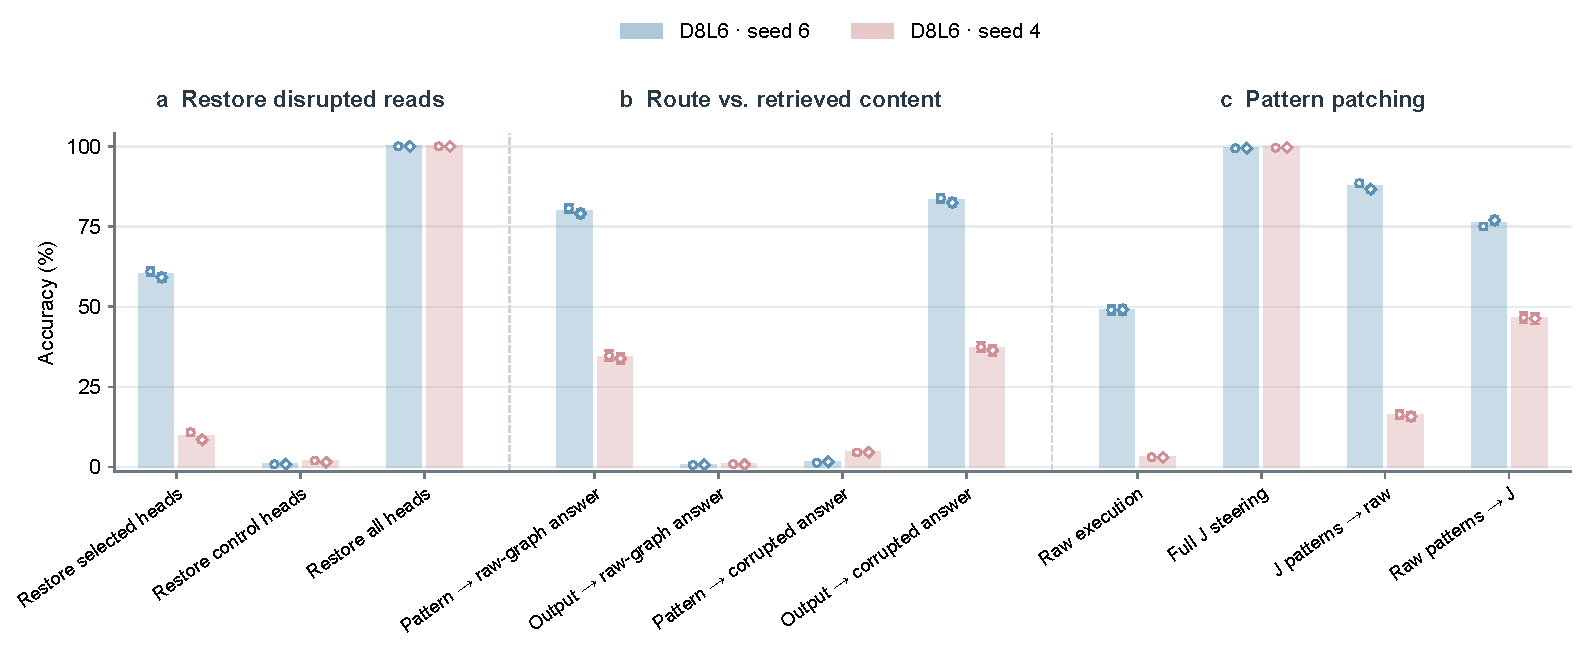
\includegraphics[width=\linewidth]{figures/fig08_graph_seeds.pdf}
\caption{Fresh confirmation of the selected D8L6 backbones on the same 512 paired graphs. Bars average two fits, with separate fit markers and 95\% graph-bootstrap intervals. Seed 6 uses H2 and seed 4 uses H3 in (a,b), with the next head modulo four as control; (c) patches all four second-layer patterns. Selection precedes this confirmation, and models are not pooled.}
\label{fig:n10-selected}\end{figure}

The seed-4 D8L6 backbone again shows that successful steering need not yield large gains from patching the tested patterns. Full steering reaches 99.6\%, while steered patterns raise unsteered accuracy from 3.0\% to 16.1\%. Restoring its selected head repairs 9.6\% of eligible broken answers, and cross-graph pattern patching selects the receiving-graph answer under the source route in 34.3\% of eligible pairs. These outcomes confirm the contrast with seed 6 without identifying the remaining pathway responsible for seed 4's successful steering.

\paragraph{Intervention scope.}
\label{app:mechanism-scope}
In D8L6, restoration and semantic patching target the selected head, while steering-pattern exchange replaces all four heads in the second layer. The smaller gains from pattern patching in other backbones therefore concern this layer-wide intervention, not a single-head exchange. Joint exchanges across graph-model layers were not tested. Ouro instead uses a sixteen-head set across three layers, specified below. In both models, source patterns come from complete runs and the receiving network continues computing after the patch. These tests identify a pathway carrying the steering effect without requiring the entire effect to pass through one head or layer.

% --- Ouro Letter-Walk ---
\section{Ouro Letter-Walk}
\label{app:parallel}
This appendix describes the language-based graph task and attention interventions used in Section~\ref{sec:hypothesis}.

\subsection{Task Definition and Input Format}
Each example defines a cycle over ten people using ten sentences of the form ``Alice passes the letter to Bob.'' The input also names the starting person and the number of steps to follow. Names are Alice, Bob, Carol, David, Emma, Frank, Grace, Henry, Iris, and Jack. Rules appear in shuffled order, so their textual order does not give the path. Ouro's tokenizer and chat template encode the instructions, rule sentences, and question as a user message. The target is an assistant message containing only the final person's name.

For example, take the cycle Alice $\to$ Bob $\to$ Carol $\to$ David $\to$ Emma $\to$ Frank $\to$ Grace $\to$ Henry $\to$ Iris $\to$ Jack $\to$ Alice. The prompt includes all ten rules. Starting with Alice, the two-step answer is \texttt{Carol} and the eight-step answer is \texttt{Iris}. A representative question from the training template is:
\begin{quote}\small
The letter starts with Alice. After exactly 02 transfers, who has it? Answer directly with only the person's name.
\end{quote}
Here ``transfers'' is the original template's word for steps; \texttt{02} is the two-digit encoding of the requested count. The rules and question are ordinary text, not one special token per person or per edge. Different prompt templates express the same task.

\subsection{Model and Steering Configuration}
\label{app:ouro-config}
\paragraph{Supervision and steering.}
Backbone fine-tuning uses requests for 1--4 steps, four recurrent loops, and answer-token cross-entropy at loop 4 only. Prompt tokens are masked from the task loss. The target includes the assistant answer and the chat-template ending, without an intermediate reasoning trace. We then freeze the backbone and fit one dense affine map on requests for 1--8 steps. The same map acts on every token before loops 2--4, and answer supervision remains at loop 4. Both stages combine task-answer cross-entropy and general-text cross-entropy with weights 0.8 and 0.2. Thus, an eight-step request is beyond backbone task training but within map training. The mechanism evaluations use eight-step questions; their attention interventions change internal activations, not the requested task or its answer rule.

\paragraph{Checkpoint and intervention sites.}
All Ouro mechanism tests use the letter-walk Ouro-2.6B checkpoint saved after 200 backbone updates and its dense affine map saved after 500 map updates. The frozen map is $J(h)=hW+b$ with unrestricted $W$, applied to all token states before loops 2--4. Head outputs are patched before their output projection during prompt processing; generation follows the receiving run's normal steering schedule.

\subsection{Evaluation and Attention Interventions}
\label{app:ouro-evaluation}
\paragraph{Head selection.}
Using zero-based layer and head indices, the selected set is L41.H2/H10/H12/H15, L43.H1/H6/H11/H13/H15, and L47.H0/H2/H3/H4/H7/H13/H15, all at loop 4. Selection begins with eight discovery pairs and uses a separate 64-pair pattern-patching confirmation set. The subsequent semantic and restoration tests keep the sixteen-head set fixed.

\paragraph{From a broad patch to a selected head set.}
The search varies late layers, neighboring-layer groups, head groups, individual head removals, and recurrent loops. A ten-head set is the primary candidate, and sixteen heads form a prespecified larger comparison. On confirmation, the ten-head set fails the criterion of retaining 90\% of the full-scope recovery; the sixteen-head set retains most of it.

The semantic and restoration experiments use sixteen comparison heads matched by layer to the selected set.

\paragraph{Restoring outputs after query replacement.}
Restoration uses 64 same-graph query pairs generated with seed 2026092701. This set is separate from localization, but was previously used for an L34.H5 restoration test. At loop 4, we replace all queries in layers 41, 43, and 47 while retaining the receiving keys and values. We then restore clean outputs at the sixteen selected heads, sixteen layer-matched comparison heads, or all 48 affected heads. Recovery conditions on clean answers broken by query replacement; restoration outcomes do not determine inclusion.

\paragraph{Pairs that separate routing from retrieved content.}
The semantic experiment draws 64 new pairs using seed 2026092901, excluding all 544 graph identities from earlier exploration, semantic and restoration panels, and localization confirmation. Each graph is a ten-person cycle. From the source starting person, the recipients at the first seven steps agree across graphs and the eighth recipient differs. The receiving query starts elsewhere. Names occupy aligned token slots.

The construction makes three answers distinct: the original receiving answer, the source answer, and the receiving-graph answer reached from the source start. A reference run with the receiving graph and source start evaluates the third answer. Pair inclusion is independent of model accuracy. This specifies the semantic predictions of pattern and head-output patching without assigning one internal loop to each task step.

\paragraph{Numerical checks and statistical reporting.}
Same-run output replacement and restoration of every affected output both yield zero maximum logit error. Pattern replacement is checked for prediction invariance, allowing floating-point differences from explicit attention reconstruction.

Ouro figure intervals are Wilson intervals. When full names are generated, we compare them with first-token predictions and count truncated generations as incorrect. The historical backbone has no verified graph-exclusion list establishing separation of these graph identities from its training set.

\subsection{Additional Results}
\label{app:ouro-results}
\paragraph{Head-output restoration.}
The table reports both accuracy over all query pairs and recovery among clean answers broken by query replacement.
\begin{table}[!htbp]\centering
\caption{Restoring Ouro head outputs at the selected positions. The last column conditions on cases broken by query replacement.}
\begin{tabular}{@{}lrr@{}}\toprule
Condition & Correct /64 & Recovered / broken\\\midrule
Clean & 63 & --- \\
Replaced queries & 0 & 0/63 \\
Selected 16 heads & 62 & 62/63 \\
Matched 16 neighbors & 1 & 1/63 \\
All 48 affected heads & 63 & 63/63 \\
\bottomrule\end{tabular}\end{table}

\paragraph{Pattern-versus-output patching.}
The table separates the original, corrupted, and rerouted answers for the same paired inputs.
\begin{table}[!htbp]\centering
\caption{Ouro pattern-versus-output patching, all 64 pairs retained. Counts use first-answer-token predictions. ``Rerouted'' means the answer obtained by following the source route on the receiving graph.}
\begin{tabular}{@{}lrrrr@{}}\toprule
Condition & Original & Source & Rerouted & Other\\\midrule
Receiving run & 61 & 0 & 1 & 2 \\
Source run & 0 & 63 & 0 & 1 \\
Receiving graph, source start & 0 & 2 & 61 & 1 \\
16-head pattern & 10 & 0 & 46 & 8 \\
16-head output & 0 & 61 & 0 & 3 \\
Matched-neighbor pattern & 61 & 0 & 1 & 2 \\
Matched-neighbor output & 61 & 0 & 1 & 2 \\
\bottomrule\end{tabular}\end{table}

For the selected sixteen heads, complete-name accuracy agrees with first-token scoring: pattern patching gives 46/64 matches to the rerouted answer and zero to the source answer; output patching gives zero and 61/64, respectively. The two interventions therefore distinguish the same answers under both scoring rules.

\paragraph{Pattern patching across head sets.}
On the 64 confirmation pairs, native and fully steered accuracy are 0/64 and 62/64. Patching steered patterns from all 256 heads over three loops into an unsteered run gives 62/64. Patching unsteered patterns into a steered run gives 0/64. The respective forward/reverse counts are 61/64 and 0/64 for sixteen heads, 50/64 and 5/64 for ten heads, and 44/64 and 12/64 for eight heads. These counts score the first answer token. Full-name generation matches them for the native, fully steered, full-scope, and ten-head conditions. Full names were not recorded for sixteen-head pattern patching, but are recorded for its later semantic and restoration tests. Localization identifies a useful head set without establishing that it is minimal.

% --- Parity ---
\section{Parity}
\label{app:parity}
This appendix defines the parity task in Section~\ref{sec:parity}, describes the readout-timing analysis, and reports results for all three backbones.

\subsection{Task Definition and Input Format}
A parity input is a sequence of binary tokens followed by a separator and, when needed, padding. The token IDs are 0 and 1 for bits, 2 for the separator, and 3 for padding. For example, the token sequence \texttt{1 0 1 1 2} has parity target 1 at the separator because it contains three ones. The sequence \texttt{1 1 0 0 2} has target 0. With batch padding, the first example can instead be \texttt{1 0 1 1 2 3 3}; the supervised output at and after the separator is then \texttt{1 3 3}. Input-bit positions are excluded from the answer loss. The semantic answer is the parity bit; the implementation also supervises the padding suffix and scores the complete answer region.

\subsection{Model and Steering Configuration}
For an input of length $n$, the loss reads the answer after $n$ loops. Backbone training uses lengths 1--20; map training freezes that backbone and uses lengths 20--40. Both use cross-entropy on the answer region. The same rank-48 diagonal-plus-low-rank affine map is applied before loops 2 through $n$. No intermediate loop is assigned a partial-parity target. The long-length experiment keeps the learned map fixed and increases both the input length and the requested loop count.

Our parity task and length-dependent loop schedule follow \citet{fan2025looped}. We use causal attention without positional encodings. Embeddings enter only at the first loop, rather than being reinjected at each loop. Three independently trained backbones are each paired with one fixed steering map.

\subsection{Evaluation and Readout-Timing Analysis}
\label{app:parity-evaluation}
\paragraph{Dense evaluation from length 500 to 1000.}
The extended curve uses seed 2's input-once backbone at update 99,000 and its map fitted on uniformly sampled lengths 20--40. We evaluate 101 lengths, $500,505,\ldots,1000$, with 128 binary inputs per length. Native and steered conditions share inputs, generated with seed $2026092401+1009n$, and retain all 12,928 sequences. Embeddings enter only at loop 1; $J$ acts before loops 2 through $n$.

Through length 500, each length uses 64 examples and the main curve uses a 10-length moving mean. From length 500 onward, every fifth length uses 128 paired examples; the dark curves average adjacent measured points, and faint points retain individual measurements. Gray shading in Figure~\ref{fig:boundary}a marks map-training lengths 20--40.

\paragraph{Heatmaps and readout offset.}
The parity heatmaps use 256 examples for each input length and loop count up to 60. Insets display lengths and loops 54--60 without interpolation; dots mark the unique best loop among $t=n-1,n,n+1$ within the measured grid. The dotted horizontal line marks the longest map-training length, $n=40$.

For each seed, the heatmaps, long-range curves, and phase measurements use the same saved map and intervention schedule. We estimate band positions using the period-four Fourier component along the offset between loop number and input length. Unwrapping the phase over input length gives a continuous band-position estimate, to which we fit a line over lengths 41--490.

Confidence intervals use 5,000 moving-block bootstrap samples of fit residuals, with block length 20. The estimate summarizes the visible accuracy bands; it does not identify an oscillator in the hidden state. The additional results below report the fitted drift, residual error, and requested-loop accuracy for all three seeds.

\subsection{Additional Results}
\label{app:parity-results}
\paragraph{Accuracy at unseen lengths.}
Table~\ref{tab:parity-uniform} reports accuracy at $t=n$ on lengths excluded from both stages of training.

\begin{table}[!htbp]
\centering
\caption{Mod-2 parity accuracy at $t=n$ (\%) on lengths excluded from both backbone and steering-map training. Each row is a separate backbone.}
\label{tab:parity-uniform}
\begin{tabular}{@{}llrr@{}}
\toprule
Protocol & Unseen lengths & Without $J$ & With $J$ \\
\midrule
Mod-2, seed 0 & 41--100 & 98.92 & 99.97 \\
Mod-2, seed 1 & 41--100 & 93.56 & 95.50 \\
Mod-2, seed 2 & 41--100 & 83.46 & 99.87 \\
\bottomrule\end{tabular}\end{table}

\paragraph{Long-range accuracy and readout timing.}
\begin{table}[!htbp]
\centering
\caption{Readout-schedule drift and longer-range accuracy with each fixed steering map. Drift is measured in loops per 100 tokens; MAE is the mean absolute deviation from the fitted phase line. Accuracy averages $t=n$ over lengths 101--500.}
\begin{tabular}{@{}lrrr@{}}
\toprule
Seed & Drift: native $\to J$ & MAE: native $\to J$ & Accuracy: native $\to J$ (\%) \\
\midrule
0 & $+0.573\to-0.327$ & $0.065\to0.069$ & $35.27\to55.71$ \\
1 & $+1.312\to+1.731$ & $0.174\to0.743$ & $44.03\to45.24$ \\
2 & $-0.961\to-0.183$ & $0.066\to0.052$ & $45.05\to73.73$ \\
\bottomrule
\end{tabular}
\end{table}

Seed 1 illustrates a difference between improving requested-loop accuracy and aligning the longer-range schedule. Its mean accuracy improves slightly, but its drift and residual error both increase with $J$, and a single linear trend poorly describes its later readouts. The complete three-seed curves below retain this variation.

% Figure 9: three parity seeds. Panel widths compensate for axis margins; retain the common alignment.
\begin{figure}[!htbp]
\centering
% Independent vector panels, assembled by LaTeX.
\setcounter{subfigure}{0}%
\begin{subfigure}[t]{0.342593\linewidth}%
\vspace{0pt}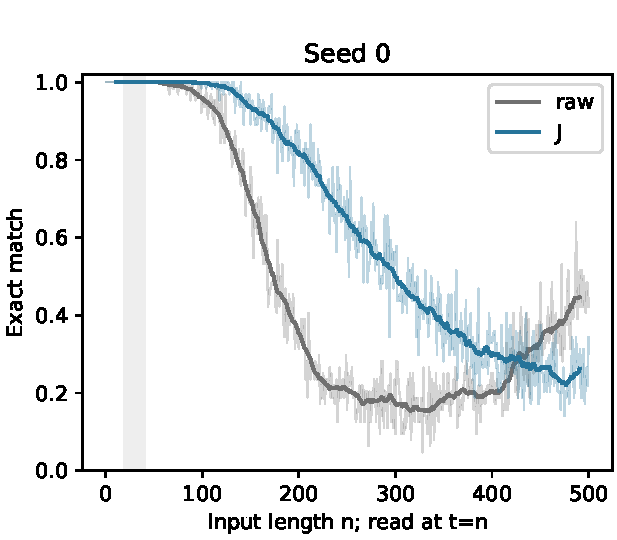
\includegraphics[width=\linewidth]{figures/fig09a_parity_seed0.pdf}%
\phantomcaption\label{fig:v64-parity_uniform_long-a}%
\end{subfigure}%
\begin{subfigure}[t]{0.327546\linewidth}%
\vspace{0pt}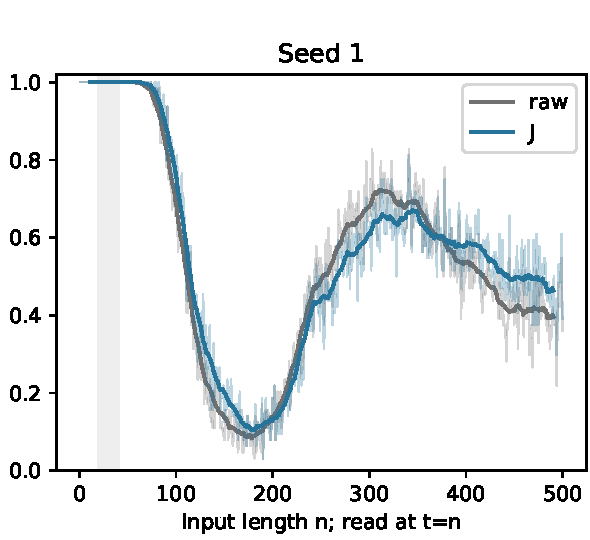
\includegraphics[width=\linewidth]{figures/fig09b_parity_seed1.pdf}%
\phantomcaption\label{fig:v64-parity_uniform_long-b}%
\end{subfigure}%
\begin{subfigure}[t]{0.329861\linewidth}%
\vspace{0pt}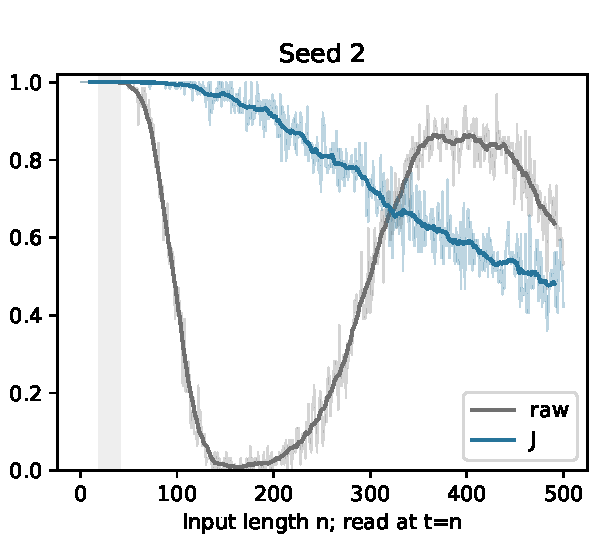
\includegraphics[width=\linewidth]{figures/fig09c_parity_seed2.pdf}%
\phantomcaption\label{fig:v64-parity_uniform_long-c}%
\end{subfigure}%

\caption{\textbf{Parity across three backbone seeds.} Each length uses 64 examples; faint lines are unsmoothed accuracies and dark lines are 20-length moving means. Gray bands indicate steering-map training lengths 20--40. These curves use the same saved steering maps as the main parity analysis.}
\end{figure}

% --- Graph Continuation ---
\section{Graph Continuation}
\label{sec:boundary}
This appendix describes the continuation experiment in Section~\ref{sec:depth-boundary}. These eight-node D8L8 models are separate from the ten-node D8L6 models used for target selection and attention interventions.

\subsection{Task Definition and Input Format}
This experiment uses the graph-token format in Appendix~\ref{app:graph-task}, with eight nodes and 29 input tokens. The query continues to specify depth 8 even when execution extends beyond eight loops. At loop $t$, the continuation target is the node reached after $t$ graph edges from the original start. The input is not rewritten with a new requested depth at each loop.

For example, on the cycle $0\to1\to\cdots\to7\to0$ with start 0, the loop-8 target is 0, the loop-9 target is 1, and the loop-10 target is 2.

\subsection{Model and Steering Configuration}
The continuation study uses twelve eight-node D8L8 backbones with seeds 100--111, separately from the ten-node D8L6 mechanism models. Each has two shared blocks, hidden width 256, and four heads, and reaches perfect endpoint accuracy at its supervised eighth loop. Two rank-48 diagonal-plus-low-rank maps are fitted for each frozen backbone using successor cross-entropy.

The backbone is trained to answer the depth request at loop 8. Map fitting instead supervises successive nodes over loops 1--16, using states generated by the steered run itself. The controller is applied before every loop, including loop 1 and evaluation loops beyond 16. This differs from the single extra loop used for D8L6 target selection.

\subsection{Evaluation Protocol}
The main evaluation draws 8,192 unique graphs uniformly without replacement from all 40,320 eight-node permutations, using seed 2026092402. It contains 993 single cycles as well as graphs with shorter cycles and fixed points. All eight starting nodes and all predictions are retained. Evaluation reuses the twelve original checkpoints and their two saved maps, with steering starting before loop 1.

Counts are stored by graph, loop, backbone, and map. We average over starting nodes and graphs, then over maps and backbones; the plotted 95\% interval bootstraps the twelve backbone means 10,000 times. Gray shading in Figure~\ref{fig:boundary}b marks loops 9--16, the displayed portion of the map-fitting range; the map remains active beyond this range. This broad sample has not been checked against historical training exclusions. The additional results below also report a separate training-excluded population.

\subsection{Additional Results}
\begin{table}[!htbp]\centering
\caption{New 8,192-graph evaluation: ordinary accuracy (\%). Each steered entry averages the two fixed steering maps; every graph and start is retained.}
\begin{tabular}{@{}lrrrr@{}}\toprule Seed & Without $J$ 9--16 & With $J$ 9--16 & Without $J$ 17--32 & With $J$ 17--32\\\midrule
100 & 31.46 & 100.00 & 34.59 & 47.01 \\
101 & 31.46 & 100.00 & 34.59 & 48.37 \\
102 & 31.46 & 99.56 & 34.59 & 45.08 \\
103 & 31.46 & 75.01 & 34.59 & 34.73 \\
104 & 31.46 & 100.00 & 34.59 & 47.09 \\
105 & 31.46 & 100.00 & 34.59 & 54.12 \\
106 & 31.46 & 99.99 & 34.59 & 50.81 \\
107 & 31.46 & 100.00 & 34.59 & 46.91 \\
108 & 31.46 & 99.93 & 34.59 & 41.09 \\
109 & 31.46 & 98.86 & 34.59 & 46.59 \\
110 & 31.46 & 88.43 & 34.59 & 39.31 \\
111 & 31.46 & 100.00 & 34.59 & 54.56 \\
\bottomrule\end{tabular}\end{table}

\paragraph{A separate training-excluded evaluation.}
A cohort of 512 graphs is excluded from backbone training, map training, and protocol selection. Its 78 single-cycle graphs give 97.42\% steered accuracy over loops 9--16 and 35.11\% over loops 17--32. Native execution averages 12.5\% in each range. All twelve backbones decline beyond the fitted range.

This subset is selected by graph structure, not successful predictions, and is reported separately from the main broad-distribution curve. Scores are computed at each loop. On an eight-node cycle, retaining one endpoint gives a correct answer once every eight loops; the resulting 12.5\% does not require sustained traversal.

% --- Ouro Antonym Cancellation ---
\section{Ouro Antonym Cancellation}
\label{app:supervision}
This appendix defines the task and the two supervision strategies compared in Section~\ref{sec:supervision-boundary}.

\subsection{Task Definition and Input Format}
The input contains a word sequence, a deletion rule, and a requested deletion count. At each step, the rule removes the leftmost adjacent antonym pair and joins the remaining words in their original order. The vocabulary consists of twelve pairs: hot/cold, near/far, open/closed, heavy/light, young/old, rich/poor, happy/sad, clean/dirty, full/empty, wet/dry, fast/slow, and alive/dead. Actual examples contain all 24 words, with pair orientations and nesting varied. Ouro encodes the full text using its tokenizer and chat template. The answer contains the two words removed at the requested step, in their left-to-right order.

A short illustrative sequence is \texttt{hot near far cold open closed}. The first deletion removes \texttt{near far}, leaving \texttt{hot cold open closed}. The second removes \texttt{hot cold}, and the third removes \texttt{open closed}. Thus, the answer to deletion 2 is \texttt{hot cold}, not the remaining sequence. This shortened example illustrates the rule; training and evaluation use 24-word inputs. In the final-only format, the question is ``Which two words are deleted on deletion number 2? Answer with only those two words in their original left-to-right order.'' The stepwise format instead states the requested number of deletions and asks for the pair removed in the current deletion update.

\subsection{Model and Steering Configuration}
\paragraph{Answer-token supervision.}
The user prompt is masked from the task loss. Cross-entropy supervises the assistant's two-word answer and chat-template ending, without a generated deletion trace.

\paragraph{Backbone supervision and request format.}
The two Ouro backbones are fine-tuned separately for 500 updates and always run for four loops. Final-only training samples requests for deletions 1--4 and supervises the requested pair at loop 4. Stepwise training supplies a prompt requesting four deletions and supervises the pair removed at deletion $t$ after loop $t$, for $t=1,\ldots,4$. The comparison therefore contrasts learning to answer a requested depth at the final loop with learning a prescribed progression of intermediate answers. The two strategies differ in both supervision and request format.

\paragraph{A shared map for each frozen backbone.}
Each backbone receives its own map $J(h)=h(I+AB)+b$, with a rank-128 residual update and 526,336 trainable parameters. It is shared across all four loops and acts on every token after each loop's RMSNorm, including after loop 4 before the frozen language-model head. Zero initialization of $B$ and $b$ makes the initial map the identity.

Both fits use 500 AdamW updates at learning rate $10^{-4}$, with 50 warmup updates. An update contains sixteen examples, two for each requested deletion depth 1--8. The loss weights answer cross-entropy by 0.8 and general-text cross-entropy by 0.2. During both map fitting and evaluation, the prompt specifies the requested deletion count. For both backbones, map training supervises the requested pair at the fixed loop-4 exit. Adaptive halting is disabled so all requests use four loops.

\subsection{Evaluation Protocol}
\paragraph{Native readout heatmaps.}
Figure~\ref{fig:ouro-native-readouts}a,b uses the trained, unsteered backbones at update 500. In the stepwise panel, the prompt requests four deletions. For each of 64 sequences, we compare the parsed pair read at each loop against each of the four true deletion pairs, producing the depth-by-loop matrix. In the final-only panel, the prompt requests the deletion depth shown on the vertical axis; each cell contains 64 examples from the archived loop-1/2 and loop-3/4 readout evaluations. These panels visualize each backbone under its native request format, rather than a matched-prompt intervention. They score the parsed deletion pair, not exact full-text generation or EOS emission.

\paragraph{Paired evaluation at deeper requested deletions.}
The main evaluation uses prompts that specify a deletion count and ask for the pair removed at that step (template 0 in the implementation). At each depth, the same 64 held-out sequence structures and target pairs are evaluated in all four conditions: each backbone with and without its map. Success requires matching the requested deletion pair. Table~\ref{tab:ouro-fixed4} gives counts at map update 500.

\subsection{Additional Results}
\paragraph{Native readouts.}
The final-only correct counts at loops 1--4, pooled over depths 1--4, are 81, 112, 255, and 256 out of 256. Early correct readouts establish earlier answer availability, rather than directly measuring the number of internal deletion operations.

\paragraph{Steering at deeper requested deletions.}
\begin{table}[!htbp]\centering
\caption{Ouro antonym-cancellation accuracy counts at a fixed four-loop exit. Each depth uses the same 64 sequences across conditions.}
\label{tab:ouro-fixed4}
\begin{tabular}{@{}lrrrr@{}}\toprule
& \multicolumn{2}{c}{Final-only} & \multicolumn{2}{c}{Stepwise}\\
Requested depth & Without $J$ & With $J$ & Without $J$ & With $J$\\\midrule
5 & 0/64 & 64/64 & 0/64 & 6/64 \\
6 & 0/64 & 62/64 & 0/64 & 6/64 \\
7 & 0/64 & 62/64 & 0/64 & 6/64 \\
8 & 0/64 & 63/64 & 0/64 & 2/64 \\
\bottomrule\end{tabular}\end{table}

Each strategy is represented by one backbone and one map. Depths 5--8 extend beyond backbone task training but are included in map fitting. The low stepwise steering accuracy establishes failure of the tested map and fitting procedure; it does not by itself prove that no alternative state intervention could elicit deeper computation.

% --- Knowledge-Graph Composition ---
\section{Knowledge-Graph Composition}
\label{app:cross-task}
This appendix describes the task and four steering-map families compared in Section~\ref{sec:complexity-boundary}.

\subsection{Task Definition and Input Format}
Each of the 16 relations is a fixed permutation of 128 entities. A relation therefore maps every entity to exactly one next entity. The world is fixed across training and evaluation; its edge table is not included in each input. The token sequence is \texttt{BOS entity relation ... relation}. Token 0 is \texttt{BOS}, entity IDs 0--127 are encoded as tokens 1--128, and relation IDs 0--15 as tokens 129--144. The target is the entity obtained by applying the listed relations in order.

For an illustrative world in which relation $r_a$ maps entity 7 to 12 and $r_b$ maps 12 to 3, \texttt{BOS e7 ra rb} has target entity 3. The shorter input \texttt{BOS e7 ra} has target 12. These symbolic names stand for single discrete tokens, not natural-language descriptions; the example mappings illustrate the task rather than quote the experimental world's permutations.

\subsection{Model and Steering Configuration}
The frozen input-once network uses two blocks, width 256, eight heads, and no positional encodings. All controller families are evaluated on this same world and backbone.

We compare affine maps with a rank-48 residual update, $J(h)=h(I+AB)+b$, dense affine maps, residual MLPs of width 256, and causal attention maps. For a composition of length $m$, execution begins with one $F$ and continues with $m-1$ repetitions of $J$ followed by $F$. The curriculum increases maximum supervised length through 4, 8, 12, 16, 20, 24, 28, and 32, allowing up to 5,000 updates per stage. Training uses truncated unrolling with an answer position that advances along the composition.

\paragraph{Readout and supervision.}
The backbone-training implementation uses short compositions of lengths 1--3, with an endpoint cross-entropy objective that reads the final relation position after the corresponding number of loops. For the controller comparison, supervision follows the composition prefixes: after loop $t$, the readout at relation position $t$ is trained to predict the entity reached after the first $t$ relations. Positions are indexed as \texttt{BOS}=0 and the starting entity=1, so this readout uses token index $t+1$. Controller loss averages these cross-entropies from step 2 onward; step 1 precedes the first controller application. Evaluation scores the final entity after all relations. No intermediate entities are supplied as input tokens.

\subsection{Evaluation Protocol}
Each evaluation cell contains 128 fresh compositions in the same world. All displayed lengths belong to the completed curriculum, so Figure~\ref{fig:steering-boundaries}d tests new compositions at trained lengths.

\subsection{Interpretation of the Controller Comparison}
There is one fit per family. Parameter count, nonlinear transformation, and token mixing vary together across these families. The comparison establishes the importance of map choice for this backbone; it neither isolates one capacity feature nor ranks the families across seeds, worlds, or unseen lengths.

\end{document}
